\section{Einleitung}

\subsection{Aufgabenstellung}

Im Rahmen dieser Arbeit wird die Implementierung einer abstrakten Datenstruktur für eine Client/Server Anwendung (siehe Abbildung \ref{fig:nachrichtendienst}) behandelt. 

Die Aufgabe dieser Anwendung ist es Tagesnachrichten von verschiedenen Redakteuren zu verwalten und in korrekter Reihenfolge an den Kunden auszuliefern. Da die Reihenfolge der Nachrichten nicht von den Redakteuren abgestimmt wird, würde diese ohne einen Zwischenserver nicht korrekt sein. Die Nachrichten werden von dem Redakteur-Client-Programm mit einer eindeutigen Nummerierung zuerst an einen Server gesendet. Dieser wird über das abstrakte Datenstruktur-Konzept einer \textit{Holdback} und \textit{Delivery Queue} verwaltet. Das heißt, dass zuerst alle Nachrichten in der \textit{Holdback Queue} gehalten und nur bei korrekter Nummer an die \textit{Delivery Queue} weitergegeben werden.\\ 
Von der \textit{Delivery Queue} aus werden die Nachrichten auf Anfrage des Lesers dann in korrekter Reihenfolge an das entsprechende Client-Programm geschickt.\\

\begin{figure}[htbp]
\begin{center}
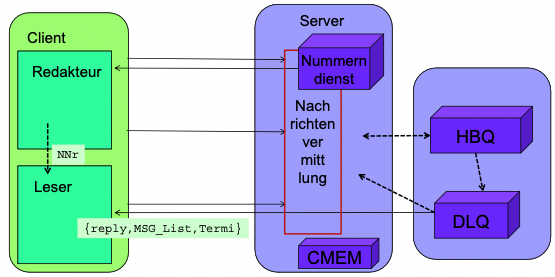
\includegraphics[scale=0.6]{Bilder/NachrichtendienstAbb.png}
\caption{\label{fig:nachrichtendienst} Nachrichtendienst \cite{Klauck2021}} 
\end{center}
\end{figure}

Da es auch hier wieder verschiedene Leser gibt hat der Server die Aufgabe sich für jeden Leser, insofern dieser sich nicht zu lange nicht mehr gemeldet hat, zu merken, welche Nachrichten er schon an diesen verschickt hat. 
Um den korrekten Ablauf der Anwendung kontrollieren zu können und um beim Implementieren Fehler möglichst einfach eliminieren zu können, werden alle Ausgaben in einer Datei \textit{HB-DLQ$<$Node$>$.log} geschrieben. Der Node auf welchem das System gerade läuft kann über den Erlang Befehl \textit{inet:gethostname()} bestimmt werden.

Da die beiden Client Programme für die Redakteure und Leser und der Server zur Verfügung gestellt wurden, wird es im folgenden um die Implementierungen der \textit{Holdback} und der \textit{Delivery Queue} gehen. Diese wird komplett in der funktionalen Programmiersprache Erlang umgesetzt.

\subsection{Funktion der Holdback Queue}

Die \textit{Holdback Queue} enthält alle Nachrichten, die nicht ausgeliefert werden dürfen. Das heißt, dass die enthaltenen Nachrichten nicht die richtigen Nummern für die \textit{Delivery Queue} haben. Durch regelmäßiges Prüfen wird entschieden, ob inzwischen eine geeignete Nachricht für die \textit{Delivery Queue} vom Server empfangen wurde. 

Da die Nachrichten nach aufsteigender Nummerierung an die \textit{Delivery Queue} weitergeleitet werden, bietet es sich an diese in der \textit{Holdback Queue} bereits zu sortieren. 
Um diese Sortierung möglichst effizient zu gestalten werden verschiedene Algorithmen getestet (siehe Kapitel \ref{Problemstellungen}.).

\subsection{Funktion der Delivery Queue}

Die \textit{Delivery Queue} ist der abstrakte Speicher für alle Nachrichten, welche an den Client ausgeliefert werden können. Die Nachrichten sind innerhalb der Queue aufsteigend sortiert. Die eigentliche Schnittstelle zum Server ist die \textit{Holdback Queue}, über diese werden die Nachrichten wieder versendet. Die \textit{Delivery Queue} ist somit lokal implementiert und wird von der \textit{Holdback Queue} aufgerufen. 

\subsection{Aufbau der Nachrichten}

Nachrichten werden von den Redakteuren entwickelt und von den Lesern konsumiert. Bis sie beim Leser ankommen, können sie aber durch mögliche Software Fehler, wie z.B. asynchrone Nebenläufigkeiten oder ähnliches, verloren gehen.\\
Die Nachrichten sind Tupel mit mindestens drei Elementen. Zum einen enthalten sie die Nachrichten-Nummer, nach welcher die Nachrichten sortiert werden. Zum anderen enthalten sie eine Textzeile in welcher die eigentliche Nachricht geschrieben steht. Abhängig davon, welche Queues sie schon durchlaufen haben, enthalten sie Zeitstempel mit den entsprechenden Eintritts- und Austrittszeiten. 

\subsection{Aufgabenerarbeitung}

Im Folgenden werden zuerst Entwürfe für die verschiedenen Queues mit ihren Funktionen erstellt, dabei wird vorerst nur die Implementierung der \textit{Holdback Queue} als Heap und die \textit{Delivery Queue} als Liste beschrieben. Die Entwürfe sollen nahe am zu implementierenden Code liegen, damit Fehler schnell eliminiert werden können. Um den Code zu testen werden Eunit Tests aus der Library \textit{'eunit/include/eunit.hrl'} geschrieben. Diese werden für spezifische Fälle angewendet, welche aus den Diagrammen der Entwürfe entschlossen werden können. Alle Elemente werden bei passender Nummerierung sofort von der \textit{Holdback} zu der \textit{Delivery Queue} weitergeleitet.
Nachdem die erste Version mit der Heapstruktur innerhalb der \textit{Holdback Queue} funktioniert, wird eine zweite mit einer Listenstruktur implementiert.
\newpage
Diese beiden zu analysieren und zu vergleichen wird der Hauptbestandteil dieser Ausarbeitung sein\footnote{Zum Analysieren werden unter anderem die Benchmarks von Matz Heitmüller genutzt.}.
Des Weiteren wird auch der Einfluss von Implementierungen mit \textit{Pattern Matching} zu welchen mit \textit{if-else Statements} verglichen. Die Messwerte Nach diesem Teil wird ein Fazit erstellt in welchem die Messergebnisse ausgewertet werden. 

\subsection{Sortierung der Nachrichten} \label{Problemstellungen}

Aufgabe dieser Hausarbeit wird das Sortieren der Nachrichten innerhalb der \textit{Holdback Queue} sein. Hierfür werden verschiedene Sortieralgorithmen getestet. Für die verschiedenen Algorithmen werden verschiedene abstrakte Datenstrukturen benötigt. So würde z.B. bei \textit{Insertion Sort} nur das Konzept der Liste, also das 'Aneinander-pipen' von Elementen, reichen. Bei einem \textit{Heap Sort} Algorithmus würde eine Heapstruktur verwendet werden müssen. Dieses Konzept basiert auf der Baumstruktur mit Wurzelknoten und Teilbäumen.\\
Hier als Beispiele drei Sortieralgorithmen (siehe Abbildung \ref{fig:sortAlgo}). Aufsteigend, absteigend und random, bezieht sich hierbei auf die Liste welche sortiert wurde.

\begin{figure}[htbp]
\begin{center}
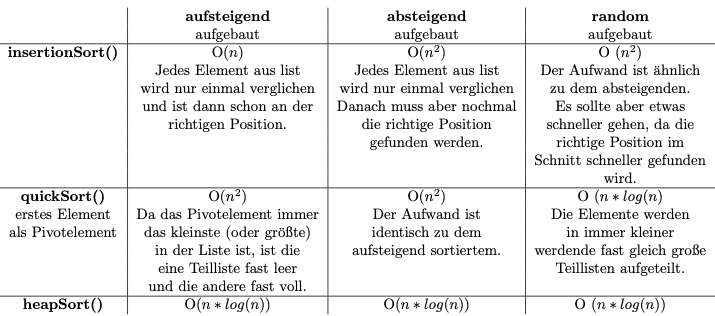
\includegraphics[scale=0.59]{Latex/Bilder/sortAlgo.png}
\caption{\label{fig:sortAlgo} Auswertung Sortieralgorithmen \cite{sortAlgo}} 
\end{center}
\end{figure}

Diese wurden bisher nur mit statischen Listen getestet. Hierbei wurde eine Liste übergeben, sortiert und der nächsten Prozess begonnen. In dieser Anwendung wird hierbei dynamisch gearbeitet. Da der \textit{Holdback Queue} frequent neue Nachrichten zugesendet werden, ist ein Algorithmus geeignet, welcher im Online-Verfahren arbeitet. Nicht alle zu sortierenden Elemente sind zu Beginn bekannt. Anbieten hierfür würde sich der \textit{InsertionSort} Algorithmus. 
Wie es der bereitgestellten logging Datei \textit{HB-DLQ@Qigong-KLC.log} (siehe Abbildung \ref{fig:HBQFilesEntry2}) zu entnehmen ist, werden die Nachrichten von den Redakteuren, mit zum größten Teil unbeständiger Nummerierung, gesendet. Für den \textit{InsertionSort} Algorithmus wäre dies aber ein Aufwand von O($n^2$).\\ Im Folgenden wird ein dem \textit{InsertionSort} ähnlicher Algorithmus verwendet. Im \textit{InsertionSort} sucht ein Laufindex das nächste unsortierte Element und fügt es an der richtigen Stelle in der Liste ein. In diesem Anwendungsfall wäre der Laufindex immer an der Position \textit{null}, da hier die neue Nachricht eingefügt wird. Der Index des Elements so lange erhöht, bis dieses die richtige Position erreicht hat. Wenn davon ausgegangen wird, dass die Elemente in zufälliger Reihenfolge eingefügt werden, entsteht eine Komplexität von $O(n/2)$. Beim Entfernen der Nachrichten gibt es in diesem Szenario den Vorteil, dass die Listen Erlang-Intern mit dem Listenkopf (Head) beginnen und an diese die restliche Liste (Tail) angehängt wird. Somit kann beim Entfernen des kleinsten Elements mit dem Tail weitergearbeitet werden, was auf einen Aufwand von $O(1)$ schließen lässt.

\begin{figure}[htbp]
\begin{center}
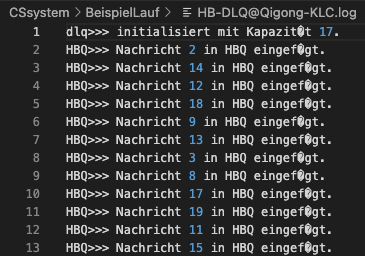
\includegraphics[scale=0.6]{Bilder/HBQFilesEntry.png}
\caption{\label{fig:HBQFilesEntry2} Nachrichtendienst \cite{HBQlogging}} 
\end{center}
\end{figure}

Der \textit{HeapSort} Algorithmus an sich setzt eine Komplexität von $O(n*log(n))$ voraus. Das liegt daran, dass die zu sortierende Liste zuerst zu einem Heap umstrukturiert werden muss. Man strukturiert den Heap in diesem Anwendungsfall von Anfang an, dadurch entfällt der Schritt. Es bleibt eine Komplexität von $O(log(n)$. Zu beachten ist, dass der Aufwand beim Einfügen und beim Entfernen auch beim Heap nicht identisch ist. Beim Einfügen gilt $O(log(n))$, da das Element eventuell nur den Heap nach oben wandert. Beim Entfernen gilt $O(2*log(n))$, da hier das Wurzelelement nach dem Entfernen ersetzt wird und der Heap somit auch neu strukturiert werden muss. Der \textit{HeapSort} Algorithmus ist bei aufsteigend sortierter Liste mit O($3*log(n)$) effizienter als der \textit{InsertionSort} Algorithmus. Mit gleichbleibender Effizienz aber deutlich besser bei random sortierter Liste. 

\subsection{Erwartungen} \label{erwartungen}

Das Ziel dieser Ausarbeitung ist es eine möglichst Effiziente Verarbeitung der Nachrichten zu erreichen. Der Fokus wird auf der Sortierung der Elemente innerhalb der \textit{Holdback Queue}, aber auch auf der Optimierung des allgemeinen Codes liegen.\\
Nach Vergleichen der beiden Implementierungen der \textit{Holdback Queue}, sollte die Sortierung über einen Heap als effizienter hervorgehen.\\
Außerdem wird geprüft, ob das Auslagern von Funktionen eine höhere Laufzeit zur Folge hat. Deswegen wird in einer Implementierung mit Hilfsfunktionen gearbeitet und in einer anderen auf diese verzichtet. Dies hat eine teilweise sehr tiefe Codestruktur und eine dementsprechend schlechte Lesbarkeit zur Folge. 
